%----------------------------------------------------------------------------
\chapter{Statisztikai hipotézisvizsgálat}

\section{Hipotézisek, próbastatisztika, kritikus tartomány}

Adott a $\mathcal{K}$ véletlen kísérlet, az $\Omega$ eseménytér,  a lehetséges valószínűségek halmaza $\mathcal{P}$ és a felette értelmezett $\mathbf{P}$ Kolmogorov-féle valószínűségi mező. Tegyük fel, hogy $\mathcal{P}$ két diszjunkt halmazra bontható: $\mathcal{P}_0$ és $\mathcal{P}_1$. Statisztikai próbát akarunk kidolgozni annak eldöntésére, hogy $H_0:\mathbf{P}\in\mathcal{P}_0$ \emph{nullhipotézis} igaz-e. Ha úgy kell döntenünk, hogy a null hipotézis nem igaz, akkor automatikusan a $H_1:\mathbf{P}\in\mathcal{P}_1$ \emph{alternatív hipotézist} fogjuk elfogadni. A döntéshez szignifikancia szintet rendelünk, amivel jellemezzük, hogy mennyire erős a döntésünk.

\emph{Kritikus érték:} $\forall \epsilon \in (0,1)$ számhoz megadhatók $K_1(\epsilon) < K_2(\epsilon)$ kritikus értékek úgy, hogy $\mathbf{P}_\nu(K_1(\epsilon)< T_n < K_2(\epsilon)) \geq 1-\epsilon$, $\nu \in \Theta_0$.

\emph{Elfogadási tartomány:} $\mathcal{X}_e = \{\underline{x} \in \mathbb{R}^n : K_1(\epsilon)< T_n < K_2(\epsilon)\}$. Ha $\underline{x} \in \mathcal{X}_e$, akkor a $H_0$ hipotézist elfogadjuk a $\epsilon$ szignifikancia-szinten ($\underline{x}$ a mintarealizáció).

\emph{Kritikus tartomány:} $\mathcal{X}_k = \mathbb{R}^n \setminus \mathcal{X}_e$


\section{Első - és másodfajú hibavalószínűség}

A döntésünk nem lesz minden esetben helyes, elképzelhető, hogy hibásan döntünk.


\begin{figure}[h]
  \caption{Heteroszkedaszticitás}
  \centering
  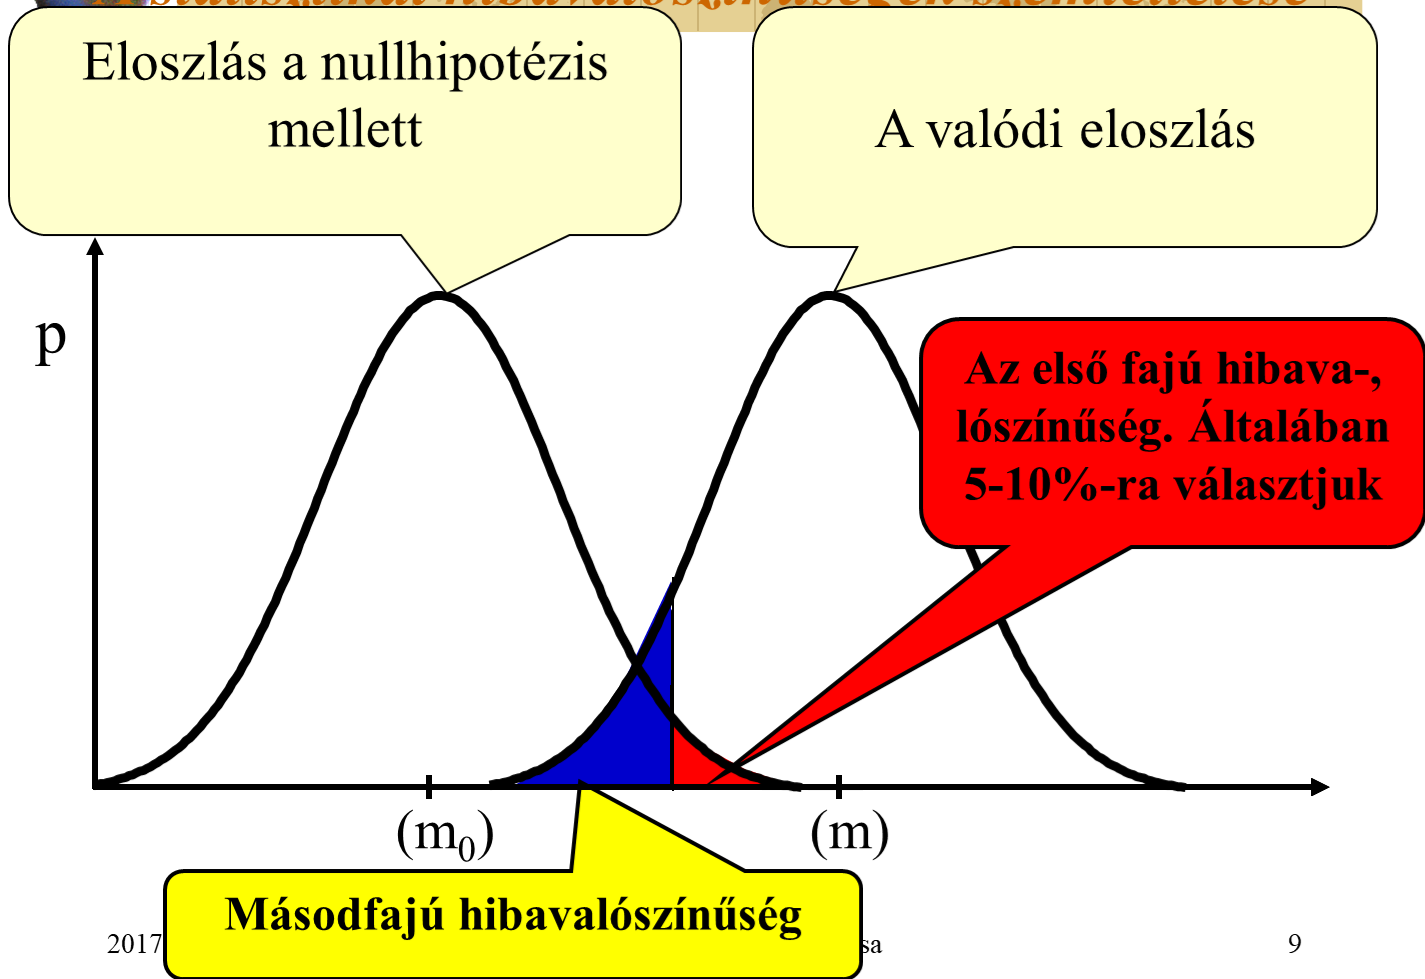
\includegraphics[width=0.7\textwidth]{figures/hibafajtak.png}
\end{figure}


\emph{Elsőfajú hiba:} $H_1$-et fogadjuk el, minközben $H_0$ igaz. Ennek értékét tudjuk befolyásolni, általában 5-10\%-ra választjuk


\emph{Másodfajú hiba:} $H_0$-t fogadjuk el, miközben $H_1$ az igaz. A másodfajú hiba értékét nehéz megállapítani

A két hibafajta között trade-offot kell találni, ha az egyiket csökkentjük, a másik nőni fog. A hibavalószínűségeket csak úgy tudjuk csökkenteni, ha növeljük a mintaelemszámot (mivel így a sűrűségfüggvények szórása csökken)

További vonatkozó tételek:
\begin{itemize}
\item \emph{Neyman-Pearson fundamentális lemma:}  Adottak a minta sűrűségfüggvényei $\mathbf{P}_0$ és $\mathbf{P}_1$ valószínűségi mértékre ($f_0$ és $f_1$), melyeknek együttes sűrűségfüggvényei $L_0$ és $L_1$. Amennyiben dönteni szeretnénk a null hipotézisről az alternatív hipotézissel szemben, akkor
\begin{itemize}
\item tetszőleges $0<\epsilon<1$ esetén $\exists c_0 >0$ és $0 < \tau < 1$ szám, amivel a \\
$\Phi(x) = 
  \begin{cases}
    1       & \quad \text{ha } L_1(x) > c_0L_0(x) \\
    \tau    & \quad \text{ha } L_1(x) = c_0L_0(x)\\
    0		& \quad \text{ha } L_1(x) < c_0L_0(x)
  \end{cases}
$
\\döntésfüggvény olyan véletlenített próbához tartozik, aminek $\epsilon$ a terjedelme
\item az előbb definiált próba egyenletesen legjobb próba
\item ha $\Phi*$ egy $\epsilon$ terjedelmű legjobb próba, akkor \\$\mathbf{P}_0(\Phi(x) = \Phi*(x))=\mathbf{P}_1(\Phi(x) = \Phi*(x))=1$
\end{itemize}
E lemma segítségével lehet rögzített elsőfajú hibavalószínűséghez a lehető legkisebbb másodfajú hibavalószínűségű próbát megkonstruálni

\item \emph{Stein-lemma:} Adottak a minta sűrűségfüggvényei $\mathbf{P}_0$ és $\mathbf{P}_1$ esetén, melyeknek relatív entrópiája $| \mathbf{D} (f_0 || f_1)| = \Big| \mathbf{E}_{\mathbf{P}_0}log_2\frac{f_0(X_1)}{f_1(X_1)} \Big|$ véges. Legyen $\alpha_n$ az elsőfajú hibavalószínűség, $\beta_n$ pedig a másodfajú hibavalószínűség. Legyen $\beta_{n,\epsilon}$, $0<\epsilon<1/2$ a legfeljebb $\epsilon$ terjedelmű próbák esetén a minimális másodfajú hibavalószínűség.\\Ekkor $lim_{n\rightarrow\infty}log_2\beta_{n,\epsilon} = - \mathbf{D} (f_0 || f_1)$
\end{itemize}

\section{Erőfüggvény, próba konzisztenciája, torzítatlansága, ereje}

\emph{Erőfüggvény: } $E(\epsilon, n, \mathbf{P}) = \mathbf{P}((X_1,X_2,...X_n)^T \in \mathcal{X}_k)$, $\mathbf{P} \in \mathcal{P}_1$, $0<\epsilon<1$, $n \in \mathbb{N}$

Próba \emph{ereje:} $\sup_{\forall \mathbf{P} \in \mathcal{P}}\mathbf{P}((X_1,X_2,...X_n)^T \in \mathcal{X}_k)$

Próba \emph{torzítatlansága:} 
\\$\mathbf{P}((X_1,X_2,...X_n)^T \in \mathcal{X}_k) \leq \epsilon$, $\forall \mathbf{P} \in \mathcal{P}_0$-ból következik, hogy \\$\mathbf{P}((X_1,X_2,...X_n)^T \in \mathcal{X}_k) \geq \epsilon$, $\forall \mathbf{P} \in \mathcal{P}_1$, $0<\epsilon<1$, vagyis ha a nullhipotézis nem áll fenn, akkor nagyobb valószínűséggel utasítjuk el, mint amikor fennáll.

Próba \emph{konzisztenciája:} $\lim_{n\rightarrow\infty}E(\epsilon, n, \mathbf{P}) = 1$, $\forall \mathbf{P} \in \mathcal{P}_1$, $0<\epsilon<1$